\chapter*{Introduction}
\addcontentsline{toc}{chapter}{Introduction} % but still display in TOC (see https://tex.stackexchange.com/a/222961)

Inspiration

\url{https://en.wikipedia.org/wiki/White_dwarf#Formation}

\url{https://en.wikipedia.org/wiki/Compact_star}

\section*{The life and death of stars}

\begin{figure}
\centering
\usetikzlibrary{positioning}
\usetikzlibrary{shapes.symbols}
\usetikzlibrary{shadows}
\usetikzlibrary{trees}
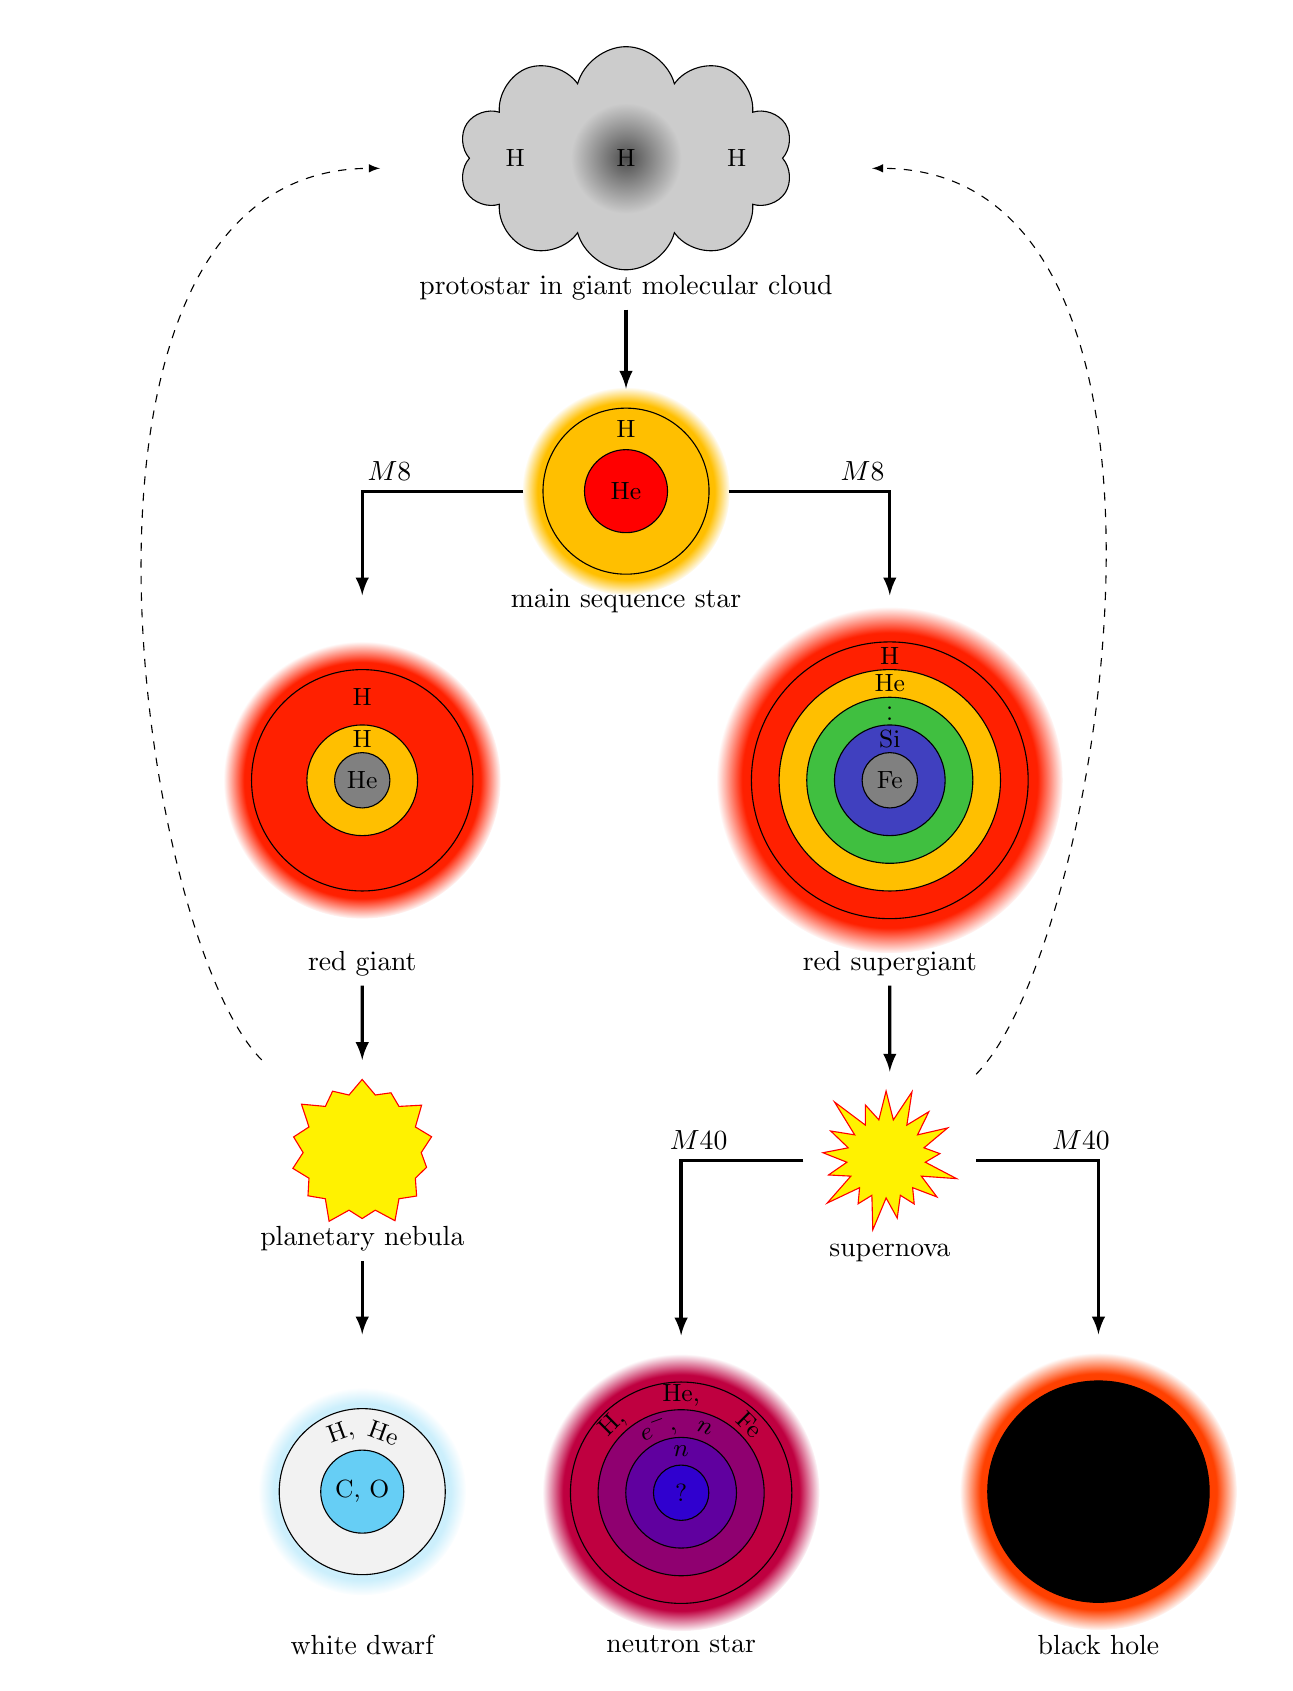
\begin{tikzpicture}[
	edge from parent/.style={draw,very thick,-latex},
	level distance=5cm,
	level 1/.style={level distance=4.1cm},
	level 2/.style={level distance=3.8cm, sibling distance=6.7cm},
	level 3/.style={level distance=4.7cm},
	level 4/.style={level distance=4.3cm, sibling distance=5.3cm},
	sibling distance=6cm,
	every label/.style={text width=4cm, text centered, inner sep=0pt, yshift=+2pt},
	element/.style={font=\small},
	dualpath/.style={
		edge from parent path={(\tikzparentnode\tikzparentanchor) -| (\tikzchildnode\tikzchildanchor)},
	},
	cloud/.pic={
		\node [draw, cloud, element, aspect=2, fill=gray, inner sep=10pt] {H};
	},
	protostar/.pic={
		\node [draw, cloud, aspect=2, fill=black!20!white, inner sep=20pt] {};
		\shade [even odd rule, inner color=black!70!white, outer color=black!20!white] circle (20pt);
		\node [element] at (0, 0) {H};
		\node [element] at (-40pt, 0) {H};
		\node [element] at (+40pt, 0) {H};
	},
	mainsequencestar/.pic={
		\draw[draw=black, fill=orange!50!yellow, circular glow={fill=orange!50!yellow}] circle [radius=30pt]; \node [element] at (90:22.5pt) {H};
		\draw[draw=black, fill=red] circle [radius=15pt]; \node [element] at (90:0pt) {He};
	},
	browndwarf/.pic={
		\filldraw[brown] circle [radius=20pt];
		\node [element] at (90:0pt) {H};
	},
	redgiant/.pic={
		\draw[draw=black, fill=red!75!orange, circular glow={fill=red!75!orange}] circle [radius=40pt]; \node [element] at (90:30pt) {H};
		\draw[draw=black, fill=orange!50!yellow] circle [radius=20pt]; \node [element] at (90:15pt) {H};
		\draw[draw=black, fill=gray] circle [radius=10pt]; \node [element] at (90: 0pt) {He};
		\draw[draw=none] (-60pt,-60pt) rectangle (+60pt,+60pt);
	},
	redsupergiant/.pic={
		\draw[draw=black, fill=red!75!orange, circular glow={fill=red!75!orange}] circle [radius=50pt]; \node [element] at (90:45pt) {H};
		\draw[draw=black, fill=orange!50!yellow] circle [radius=40pt]; \node [element] at (90:35pt) {He};
		\draw[draw=black, fill=green!50!gray] circle [radius=30pt]; \node [element] at (90:25pt) {$\vdots$ };
		\draw[draw=black, fill=blue!50!gray] circle [radius=20pt]; \node [element] at (90:15pt) {Si};
		\draw[draw=black, fill=gray] circle [radius=10pt]; \node [element] at (90:0pt) {Fe};
		\draw[draw=none] (-60pt,-60pt) rectangle (+60pt,+60pt);
	},
	supernova/.pic={
		\node[starburst, fill=yellow, draw=red, minimum size=2cm] {};
	},
	planetarynebula/.pic={
		\node[starburst, starburst points=14, starburst point height=0.25cm, fill=yellow, draw=red,  minimum size=2.0cm] {};
	},
	blackhole/.pic={
		\draw [fill=black, circular glow={fill=red!50!orange}] circle[radius=40pt];
		\draw[draw=none] (-50pt, -50pt) rectangle (+50pt, +50pt);
	},
	neutronstar/.pic={
		\draw[draw=black, fill=blue!  0!purple, circular glow={fill=blue!0!purple}] circle [radius=40pt]; \node [element, rotate=45] at (135:35pt) {H,}; \node [element] at ( 90:35pt) {He,}; \node [element, rotate=-45] at (45:35pt) {Fe};
		\draw[draw=black, fill=blue! 25!purple] circle [radius=30pt]; \node [element, rotate=+20] at (110:25pt) {$e^-$,}; \node [element, rotate=-20] at (70:25pt) {$n$};
		\draw[draw=black, fill=blue! 50!purple] circle [radius=20pt]; \node [element] at (90:15pt) {$n$};
		\draw[draw=black, fill=blue! 75!purple] circle [radius=10pt]; \node [element] at (90: 0pt) {?};
		\draw[draw=none] (-50pt, -50pt) rectangle (+50pt, +50pt);
	},
	whitedwarf/.pic={
		\draw[draw=black, fill=white! 90!gray, circular glow={fill=cyan! 20!white}] circle [radius=30pt]; \node [element, rotate=+20] at (110:22.5pt) {H,}; \node [element, rotate=-20] at (70:22.5pt) {He};
		\draw[draw=black, fill=cyan! 60!white] circle [radius=15pt]; \node [element] at (90:0pt) {C, O};
		\draw[draw=none] (-50pt, -50pt) rectangle (+50pt, +50pt);
	},
]

	\node (protostar) {\tikz \node [label={[text width=6.0cm]below:\subcaption{\label{fig:intro:star_evolution_protostar}protostar in giant molecular cloud}}] {\tikz \pic {protostar};};}
		child { node [label={[]below:\subcaption{\label{fig:intro:star_evolution_mainseq}main sequence star}}] {\tikz \node [] {\tikz \pic {mainsequencestar};};}
			child { node {\tikz \node [label={below:\subcaption{\label{fig:intro:star_evolution_red_giant}red giant}}] {\tikz \pic {redgiant};};}
				child { node (planetarynebula) {\tikz \node [label={below:\subcaption{\label{fig:intro:star_evolution_planetary_nebula}planetary nebula}}] {\tikz \pic {planetarynebula};};}
					child { node {\tikz \node [label={below:\subcaption{\label{fig:intro:star_evolution_white_dwarf}white dwarf}}] {\tikz \pic {whitedwarf};};} }
				} edge from parent [dualpath] node [above, anchor=south west, xshift=-2pt] {$M \lesssim 8 \solarmass$}
			}
			child { node {\tikz \node [label={below:\subcaption{\label{fig:intro:star_evolution_red_supergiant}red supergiant}}] {\tikz \pic {redsupergiant};};}
				child { node (supernova) [label={below:\subcaption{\label{fig:intro:star_evolution_supernova}supernova}}] {\tikz \node [] {\tikz \pic {supernova};};}
					child { node {\tikz \node [label={below:\subcaption{\label{fig:intro:star_evolution_neutron_star}neutron star}}] {\tikz \pic {neutronstar};};} edge from parent [dualpath] node[above, anchor=south west, xshift=-8pt] {$M \lesssim 40 \solarmass$} }
					child { node {\tikz \node [label={below:\subcaption{\label{fig:intro:star_evolution_black_hole}black hole}}] {\tikz \pic {blackhole};};} edge from parent [dualpath] node[above, anchor=south east, xshift=+8pt] {$M \gtrsim 40 \solarmass$} }
				}
				edge from parent [dualpath] node [above, anchor=south east, xshift=+2pt] {$M \gtrsim 8 \solarmass$}
			}
		};
	\draw [-latex, dashed] (supernova)       to [out= 45, in=  0, out looseness=0.5] (protostar);
	\draw [-latex, dashed] (planetarynebula) to [out=135, in=180, out looseness=0.5] (protostar);
\end{tikzpicture}
\caption{\label{fig:intro:star_evolution}%
	A simplified life cycle of stars and their main structure at every stage (not to scale).
}
\end{figure}

% planetary nebula -> releases ionized gas -> forms clouds
The mothers of all stars are enormous accumulations of light elements like hydrogen called \textbf{giant molecular clouds}, formed by the ashes of dying stars whose life cycle we are about to describe.
Such clouds consist of matter weighing between tens of thousands to tens of millions solar masses, distributed with a relatively low average density over a huge area that are tens to hundreds of lightyears across.
Internally, the dynamics of a molecular cloud is, most importantly, governed by the attractive force of gravity between particles and the repulsive thermal pressure from their thermal motion and collisions.

Due to the force of gravity, parts of the cloud can clump together in areas of greater density.
The larger the mass, the more surrounding material is attracted, causing the clump to grow like a rolling snowball.
Initially, the density is low and thermal radiation can escape from the X.
As the density increases, however, thermal radiation can no longer find its way out and is trapped.
The temperature therefore increases, and so does the pressure.
As the clump continues to grow in mass by sucking up surrounding material, becoming ever denser and hotter, it receives the more honorable name \textbf{protostar}.

At some point, the temperature has become so high that hydrogen can fuse to form helium.
This greatly increases the pressure, and the protostar ultimately stops contracting and reaches a state of equilibrium and has become a grown-up \textbf{main sequence star}.
In this stage, fusion of hydrogen into helium continues -- the heavier helium is pulled into the central regions of the star and is called the \emph{core}, while the lighter hydrogen contitutes an outer shell.
What happens next depends heavily on the mass of the star.

If the star is not so massive, the fusion stops with helium, and as hydrogen is depleted, the supporting pressure falls and the star begins to contract again, causing the temperature to rise again.
The core collapses, while the temperature in the outer hydrogen layer can increase so that hydrogen begins to burn again, causing the outer parts of the star to expand, and the star is a \textbf{red giant}.
As the core continues to heat up, it may eventually reach $10^8 K$, where helium fuses into carbon, causing an explosive reaction, the envelope becomes unstable and the outer parts of the star is expelled in a \textbf{planetary nebula}, while the core remains as a \textbf{white dwarf}, supported by the degeneracy pressure of electrons, maximum mass Chandrasekhar mass $1.4$?

If the star is more massive, fusion continues all the way until hydrogen and the star becomes a \textbf{red supergiant}.
It eventually explodes in a \textbf{supernova}, and the core collpases to a \textbf{neutron star}.
The equilibrium configuration of a neutron star is composed of neutrons, protons, hyperons, leptons and possibly quarks.

\section*{Neutron stars}


Since the dawn of mankind, humans have gazed upon the night sky with great curiosity of what lies out in the universe.
\begin{itemize}
\item Establish the importance of studying stars from an existential point of view.
\item Give a brief historical review of how our view of stars and the universe has changed, from the nonscientific views of the earliest days to the scientific viewpoint of the modern age.
\end{itemize}

After the discovery of the neutron in 1933, scientists soon proposed the existence of stars consisting of neutrons.
\begin{itemize}
\item Explain why neutron stars are plausible, from the original ``ignorant'' point of view before one has a good theoretical understanding of neutron stars.
\item Review the hypotheses that came from the initial theoretical work on neutron stars, before any observation was made.
\end{itemize}

In 1967, Jocelyn Bell and Antony Hewish discovered the first known neutron star.
\begin{itemize}
\item Review observations that have been made from neutron stars up until today.
\item Connect the observations made to the theoretical hypotheses from the last paragraph.
\end{itemize}

Today, scientists have a good understanding of neutron stars.
\begin{itemize}
\item Explain the modern, ``perfect'' understanding of neutron stars, that have not been covered by the ``naive'' view in the last two paragraphs.
\item Explain that neutron stars are formed by supernova explosions.
\item Explain that neutron stars are the smallest and densest class of stars that have been observed.
\item Explain that neutron stars are kept stable by the balance between gravitational attraction and Pauli pressure.
\end{itemize}

Being one of the most exotic types of objects humanity has observed, neutron stars are a gateway to developing our understanding of new, hypothetical astronomical objects.
\begin{itemize}
\item Explain why it is important to understand neutron stars first (even if others already understand them), in order to do new and interesting work.
\item Explain the possibility that neutron stars can develop into even more, currently hypothetical classes of stars, such as quark stars.
\end{itemize}

\section*{Outline of this thesis}

In this thesis, we develop the theoretical tools necessary to study stars made of free neutrons, calculate their mass-radius curve and study their stability.
\begin{itemize}
\item State the content of this thesis, distinguishing between the theoretical tools we develop, and the results that we obtain by calculations with these tools.
\item Although these are not new findings but rather a review, this is our ``niche''.
\item To ``occupy our niche'', this paragraph should explain \emph{why} this particular content is the most natural buildup for a thesis on neutron stars.
\end{itemize}

In \textbf{\cref{chap:tov}}, we derive the \textbf{Tolman-Oppenheimer-Volkoff system of equations}
\begin{align*}
	\odv{P}{r} &= -\frac{G m \epsilon}{r^2 c^2} \left( 1 + \frac{P}{\epsilon} \right) \left( 1 + \frac{4 \pi r^3 P}{m c^2} \right) \left( 1 - \frac{2 G m}{r c^2} \right)^{-1} , \\
	\odv{m}{r} &= \frac{4 \pi r^2 \epsilon}{c^2} ,
\end{align*}
from the theory of general relativity.
\begin{itemize}
\item Explain why Newtonian gravity does not suffice to study stars, and that the relativistic effects of Einstein's theory is needed.
\item Explain the importance of the TOV equations for the study of \emph{any} kind of star.
\item Explain that the three unknowns in the equation are the pressure $P$, mass $m$ and energy density $\epsilon$.
      Since there are only two equations, we must find an additional one to solve for the unknowns.
      This is the equation of state $\epsilon = \epsilon(P)$, which is outside the scope of general relativity and must be found by statistical physics and quantum theory.
\end{itemize}

In \textbf{\cref{chap:tft}}, we will study \textbf{thermal field theory} -- the formalism needed to find the effects of quantum fields at nonzero temperature.
\begin{itemize}
\item Explain that thermal field theory is the ``missing link'' needed to find $\epsilon$ in the Tolman-Oppenheimer-Volkoff equation.
\item Present the buildup of this chapter: the partition function is needed for finding expectation values of thermodynamic variables, the partition function can be found by a path integral.
\item We first show how one does the path integral for bosons with complex numbers, then introduce anticommuting Grassmann numbers to find the path integral for fermions.
\end{itemize}

In \textbf{\cref{chap:nstars}}, we finally put together the pieces of \cref{chap:tov} and \cref{chap:tft} and study \textbf{neutron stars}.
\begin{itemize}
\item Make very clear that while chapter 1 and 2 ``only'' develop theoretical tools, chapter 1+2=3 puts the tools to work together and constitutes our ``results'' chapter.
\item Having found the partition function for free fermions in \cref{chap:tft}, we find the equation of state $\epsilon = \epsilon(P)$ for a gas of free neutrons.
\item Then we insert the equation of state into the Tolman-Oppenheimer-Volkoff equations and solve them, which yield the mass-radius-curve of neutron stars parametrized by their central pressure.
\item This is our ``results'', then we compare them to observations and earlier theoretical work.
\item Finally, we study the stability of the stars we have found.
\end{itemize}

In \textbf{\cref{chap:gr}}, we give a comprehensive \textbf{review of the theory of general relativity}.
\begin{itemize}
\item Say that this appendix enables readers unfamiliar with general relativity to understand all aspects of it that are needed for our purposes.
\end{itemize}

In \textbf{\cref{chap:relfluid}}, we study \textbf{relativistic fluid mechanics}.
\begin{itemize}
\item Assuming familiarity with general relativity, we derive all results needed to study the stability of stars.
\end{itemize}

In \textbf{\cref{chap:matsum}}, we describe the technique of \textbf{Matsubara frequency summation}.
\begin{itemize}
\item This is an elegant mathematical tool that is extremely useful to perform calculations in thermal field theory.
\item Say that this summation on its own is purely mathematical, and that the results thereof can be considered as mathematical identities only, when they are applied in the chapter on thermal field theory.
\item However, note that the results of the mathematical identities are of great physical interest, as it is precisely these identities that give rise to the bosonic and fermionic distributions.
\end{itemize}

In \textbf{\cref{chap:integrals}}, we list all integrals used throughout this thesis with pure proofs.

In \textbf{\cref{chap:code}}, we list all source code used for numerical work in this thesis.
